%!TEX TS-program = xelatex
%!TEX encoding = UTF-8 Unicode

%% document settings
\documentclass[10pt]{article}\usepackage[]{graphicx}\usepackage[]{color}
% maxwidth is the original width if it is less than linewidth
% otherwise use linewidth (to make sure the graphics do not exceed the margin)
\makeatletter
\def\maxwidth{ %
  \ifdim\Gin@nat@width>\linewidth
    \linewidth
  \else
    \Gin@nat@width
  \fi
}
\makeatother

\definecolor{fgcolor}{rgb}{0.345, 0.345, 0.345}
\newcommand{\hlnum}[1]{\textcolor[rgb]{0.686,0.059,0.569}{#1}}%
\newcommand{\hlstr}[1]{\textcolor[rgb]{0.192,0.494,0.8}{#1}}%
\newcommand{\hlcom}[1]{\textcolor[rgb]{0.678,0.584,0.686}{\textit{#1}}}%
\newcommand{\hlopt}[1]{\textcolor[rgb]{0,0,0}{#1}}%
\newcommand{\hlstd}[1]{\textcolor[rgb]{0.345,0.345,0.345}{#1}}%
\newcommand{\hlkwa}[1]{\textcolor[rgb]{0.161,0.373,0.58}{\textbf{#1}}}%
\newcommand{\hlkwb}[1]{\textcolor[rgb]{0.69,0.353,0.396}{#1}}%
\newcommand{\hlkwc}[1]{\textcolor[rgb]{0.333,0.667,0.333}{#1}}%
\newcommand{\hlkwd}[1]{\textcolor[rgb]{0.737,0.353,0.396}{\textbf{#1}}}%
\let\hlipl\hlkwb

\usepackage{framed}
\makeatletter
\newenvironment{kframe}{%
 \def\at@end@of@kframe{}%
 \ifinner\ifhmode%
  \def\at@end@of@kframe{\end{minipage}}%
  \begin{minipage}{\columnwidth}%
 \fi\fi%
 \def\FrameCommand##1{\hskip\@totalleftmargin \hskip-\fboxsep
 \colorbox{shadecolor}{##1}\hskip-\fboxsep
     % There is no \\@totalrightmargin, so:
     \hskip-\linewidth \hskip-\@totalleftmargin \hskip\columnwidth}%
 \MakeFramed {\advance\hsize-\width
   \@totalleftmargin\z@ \linewidth\hsize
   \@setminipage}}%
 {\par\unskip\endMakeFramed%
 \at@end@of@kframe}
\makeatother

\definecolor{shadecolor}{rgb}{.97, .97, .97}
\definecolor{messagecolor}{rgb}{0, 0, 0}
\definecolor{warningcolor}{rgb}{1, 0, 1}
\definecolor{errorcolor}{rgb}{1, 0, 0}
\newenvironment{knitrout}{}{} % an empty environment to be redefined in TeX

\usepackage{alltt}
\usepackage{euler}
\usepackage{xunicode,xltxtra}
\usepackage{fontspec}

\usepackage[a4paper, margin = 1 in, left = .5 in, right = .5 in]{geometry}

\usepackage{setspace}
\usepackage[dvipsnames]{xcolor}

% fonts
	\defaultfontfeatures{Mapping=tex-text, Ligatures=TeX}
	\setromanfont[Mapping=tex-text, Numbers={Proportional}]{Linux Biolinum}
	\setsansfont[Scale=MatchLowercase,Mapping=tex-text]{Optima}
	\setmonofont[Scale=MatchLowercase]{Andale Mono}

\usepackage{amsmath}
\usepackage{amssymb}
% \usepackage{mathtools}
\usepackage{linguex}
\usepackage{booktabs}

\usepackage[colorlinks=true,citecolor=MidnightBlue,urlcolor=MidnightBlue,linkcolor=MidnightBlue]{hyperref}

\title{Effects on projectivity ratings by Embedding Operator and Trigger --- \newline Data Analysis}
\author{Lisa Hofmann}
\date{\today}
\IfFileExists{upquote.sty}{\usepackage{upquote}}{}
\begin{document}
\setkeys{Gin}{width=1.0\textwidth}


\maketitle
\setcounter{tocdepth}{2}
\tableofcontents

\section{Introducing the dataset}


\begin{knitrout}
\definecolor{shadecolor}{rgb}{0.969, 0.969, 0.969}\color{fgcolor}\begin{kframe}
\begin{alltt}
\hlstd{> }\hlkwd{str}\hlstd{(data)}
\end{alltt}
\begin{verbatim}
'data.frame':	57160 obs. of  9 variables:
 $ workerid     : int  1 1 1 1 1 1 1 1 1 1 ...
 $ content      : chr  "charley" "danny" "emily" "emma" ...
 $ short_trigger: chr  "acknowledge" "hear" "reveal" "discover" ...
 $ ai_block     : chr  "block1" "block1" "block1" "block1" ...
 $ ai           : num  0.98 0.99 0.99 0.99 0.98 0.98 1 0.99 0.99 0.99 ...
 $ projective   : num  0.3 0.98 0.01 0.99 0.98 0.99 0.01 0.01 0.27 0.01 ...
 $ verb         : chr  "acknowledge" "hear" "reveal" "discover" ...
 $ op           : chr  "q" "q" "q" "q" ...
 $ exp_block    : int  1 1 1 1 1 1 1 1 1 1 ...
\end{verbatim}
\begin{alltt}
\hlstd{> }\hlstd{data}\hlopt{$}\hlstd{workerid} \hlkwb{<-} \hlkwd{as.factor}\hlstd{(data}\hlopt{$}\hlstd{workerid)}
\hlstd{> }\hlkwd{length}\hlstd{(}\hlkwd{levels}\hlstd{(data}\hlopt{$}\hlstd{workerid))}
\end{alltt}
\begin{verbatim}
[1] 2682
\end{verbatim}
\end{kframe}
\end{knitrout}


\noindent The dataset consists of $57160$ observations from $2682$ participants (recruited on the online platforms Prolific and Amazon Mechanical Turk), across 12 experiments.

We are interested in how highly participants rate speaker commitment to the truth of an embedded complement clause, coded as \texttt{projective} on a real-numbered sliding scale between $0-1$.\\

\noindent The complement clause was embedded under an attitude verb, which in turn was embedded under an entailment-cancelling operator. Our fixed effects factors manipulate the following:

\begin{enumerate}
  \item The choice of attitude verb (coded as \texttt{verb})
  \item The entailment-cancelling operator (coded as \texttt{op})
\end{enumerate}

\noindent The levels for our fixed effects factors are the following:
\begin{knitrout}
\definecolor{shadecolor}{rgb}{0.969, 0.969, 0.969}\color{fgcolor}\begin{kframe}
\begin{alltt}
\hlstd{> }\hlstd{data}\hlopt{$}\hlstd{verb} \hlkwb{<-} \hlkwd{as.factor}\hlstd{(data}\hlopt{$}\hlstd{verb)}
\hlstd{> }\hlkwd{levels}\hlstd{(data}\hlopt{$}\hlstd{verb)}
\end{alltt}
\begin{verbatim}
 [1] "acknowledge" "admit"       "announce"    "be_annoyed"  "be_right"   
 [6] "confess"     "confirm"     "demonstrate" "discover"    "establish"  
[11] "hear"        "inform"      "know"        "pretend"     "prove"      
[16] "reveal"      "say"         "see"         "suggest"     "think"      
\end{verbatim}
\begin{alltt}
\hlstd{> }\hlkwd{length}\hlstd{(}\hlkwd{levels}\hlstd{(data}\hlopt{$}\hlstd{verb))}
\end{alltt}
\begin{verbatim}
[1] 20
\end{verbatim}
\begin{alltt}
\hlstd{> }\hlstd{data}\hlopt{$}\hlstd{op} \hlkwb{<-} \hlkwd{as.factor}\hlstd{(data}\hlopt{$}\hlstd{op)}
\hlstd{> }\hlkwd{levels}\hlstd{(data}\hlopt{$}\hlstd{op)}
\end{alltt}
\begin{verbatim}
[1] "c" "m" "n" "q"
\end{verbatim}
\begin{alltt}
\hlstd{> }\hlkwd{length}\hlstd{(}\hlkwd{levels}\hlstd{(data}\hlopt{$}\hlstd{op))}
\end{alltt}
\begin{verbatim}
[1] 4
\end{verbatim}
\end{kframe}
\end{knitrout}

\noindent We are interested in the effect on \texttt{projective} of \texttt{verb} and \texttt{op}, as well as their interaction, corresponding to a $20 \times 4$ factorial design, yielding
\begin{knitrout}
\definecolor{shadecolor}{rgb}{0.969, 0.969, 0.969}\color{fgcolor}\begin{kframe}
\begin{alltt}
\hlstd{> }\hlkwd{length}\hlstd{(}\hlkwd{levels}\hlstd{(data}\hlopt{$}\hlstd{verb))}\hlopt{*}\hlkwd{length}\hlstd{(}\hlkwd{levels}\hlstd{(data}\hlopt{$}\hlstd{op))}
\end{alltt}
\begin{verbatim}
[1] 80
\end{verbatim}
\end{kframe}
\end{knitrout}
conditions.\\

\noindent We have $20$ items, corresponding to the content of the complement clause.
\begin{knitrout}
\definecolor{shadecolor}{rgb}{0.969, 0.969, 0.969}\color{fgcolor}\begin{kframe}
\begin{alltt}
\hlstd{> }\hlstd{data}\hlopt{$}\hlstd{content} \hlkwb{<-} \hlkwd{as.factor}\hlstd{(data}\hlopt{$}\hlstd{content)}
\hlstd{> }\hlkwd{levels}\hlstd{(data}\hlopt{$}\hlstd{content)}
\end{alltt}
\begin{verbatim}
 [1] "charley"  "danny"    "emily"    "emma"     "frank"    "grace"   
 [7] "isabella" "jackson"  "jayden"   "jon"      "josh"     "josie"   
[13] "julian"   "mary"     "mia"      "olivia"   "owen"     "sophia"  
[19] "tony"     "zoe"     
\end{verbatim}
\begin{alltt}
\hlstd{> }\hlkwd{length}\hlstd{(}\hlkwd{levels}\hlstd{(data}\hlopt{$}\hlstd{content))}
\end{alltt}
\begin{verbatim}
[1] 20
\end{verbatim}
\end{kframe}
\end{knitrout}

\noindent We have roughly $36$ observations by item and condition. This is an approximate number, because the \texttt{op} manipulation is a between-studies manipulation, and the number of participants differs by experiment:
\begin{knitrout}
\definecolor{shadecolor}{rgb}{0.969, 0.969, 0.969}\color{fgcolor}\begin{kframe}
\begin{alltt}
\hlstd{> }\hlcom{# n observations}
\hlstd{> }\hlkwd{length}\hlstd{(data[,}\hlnum{1}\hlstd{])}
\end{alltt}
\begin{verbatim}
[1] 57160
\end{verbatim}
\begin{alltt}
\hlstd{> }\hlcom{# observations by item}
\hlstd{> }\hlkwd{length}\hlstd{(data[,}\hlnum{1}\hlstd{])}\hlopt{/}\hlkwd{length}\hlstd{(}\hlkwd{levels}\hlstd{(data}\hlopt{$}\hlstd{content))}
\end{alltt}
\begin{verbatim}
[1] 2858
\end{verbatim}
\begin{alltt}
\hlstd{> }\hlkwd{table}\hlstd{(data}\hlopt{$}\hlstd{content)}
\end{alltt}
\begin{verbatim}

 charley    danny    emily     emma    frank    grace isabella  jackson 
    2858     2858     2858     2858     2858     2858     2858     2858 
  jayden      jon     josh    josie   julian     mary      mia   olivia 
    2858     2858     2858     2858     2858     2858     2858     2858 
    owen   sophia     tony      zoe 
    2858     2858     2858     2858 
\end{verbatim}
\begin{alltt}
\hlstd{> }\hlcom{# observations by verb}
\hlstd{> }\hlkwd{length}\hlstd{(data[,}\hlnum{1}\hlstd{])}\hlopt{/}\hlkwd{length}\hlstd{(}\hlkwd{levels}\hlstd{(data}\hlopt{$}\hlstd{verb))}
\end{alltt}
\begin{verbatim}
[1] 2858
\end{verbatim}
\begin{alltt}
\hlstd{> }\hlkwd{table}\hlstd{(data}\hlopt{$}\hlstd{verb)}
\end{alltt}
\begin{verbatim}

acknowledge       admit    announce  be_annoyed    be_right     confess 
       2858        2858        2858        2858        2858        2858 
    confirm demonstrate    discover   establish        hear      inform 
       2858        2858        2858        2858        2858        2858 
       know     pretend       prove      reveal         say         see 
       2858        2858        2858        2858        2858        2858 
    suggest       think 
       2858        2858 
\end{verbatim}
\begin{alltt}
\hlstd{> }\hlcom{# observations by operator}
\hlstd{> }\hlkwd{length}\hlstd{(data[,}\hlnum{1}\hlstd{])}\hlopt{/}\hlkwd{length}\hlstd{(}\hlkwd{levels}\hlstd{(data}\hlopt{$}\hlstd{op))}
\end{alltt}
\begin{verbatim}
[1] 14290
\end{verbatim}
\begin{alltt}
\hlstd{> }\hlkwd{table}\hlstd{(data}\hlopt{$}\hlstd{op)}
\end{alltt}
\begin{verbatim}

    c     m     n     q 
14400 14680 14340 13740 
\end{verbatim}
\begin{alltt}
\hlstd{> }\hlcom{# observations by item and condition}
\hlstd{> }\hlkwd{length}\hlstd{(data[,}\hlnum{1}\hlstd{])}\hlopt{/}\hlkwd{length}\hlstd{(}\hlkwd{levels}\hlstd{(data}\hlopt{$}\hlstd{content))}\hlopt{/}
\hlstd{+ }  \hlstd{(}\hlkwd{length}\hlstd{(}\hlkwd{levels}\hlstd{(data}\hlopt{$}\hlstd{verb))}\hlopt{*}\hlkwd{length}\hlstd{(}\hlkwd{levels}\hlstd{(data}\hlopt{$}\hlstd{op)))}
\end{alltt}
\begin{verbatim}
[1] 35.725
\end{verbatim}
\end{kframe}
\end{knitrout}

\newpage
\section{Data Overview and Statistical Summaries}
\subsection{Distribution of projectivity ratings by operator:}
\begin{knitrout}
\definecolor{shadecolor}{rgb}{0.969, 0.969, 0.969}\color{fgcolor}

{\centering 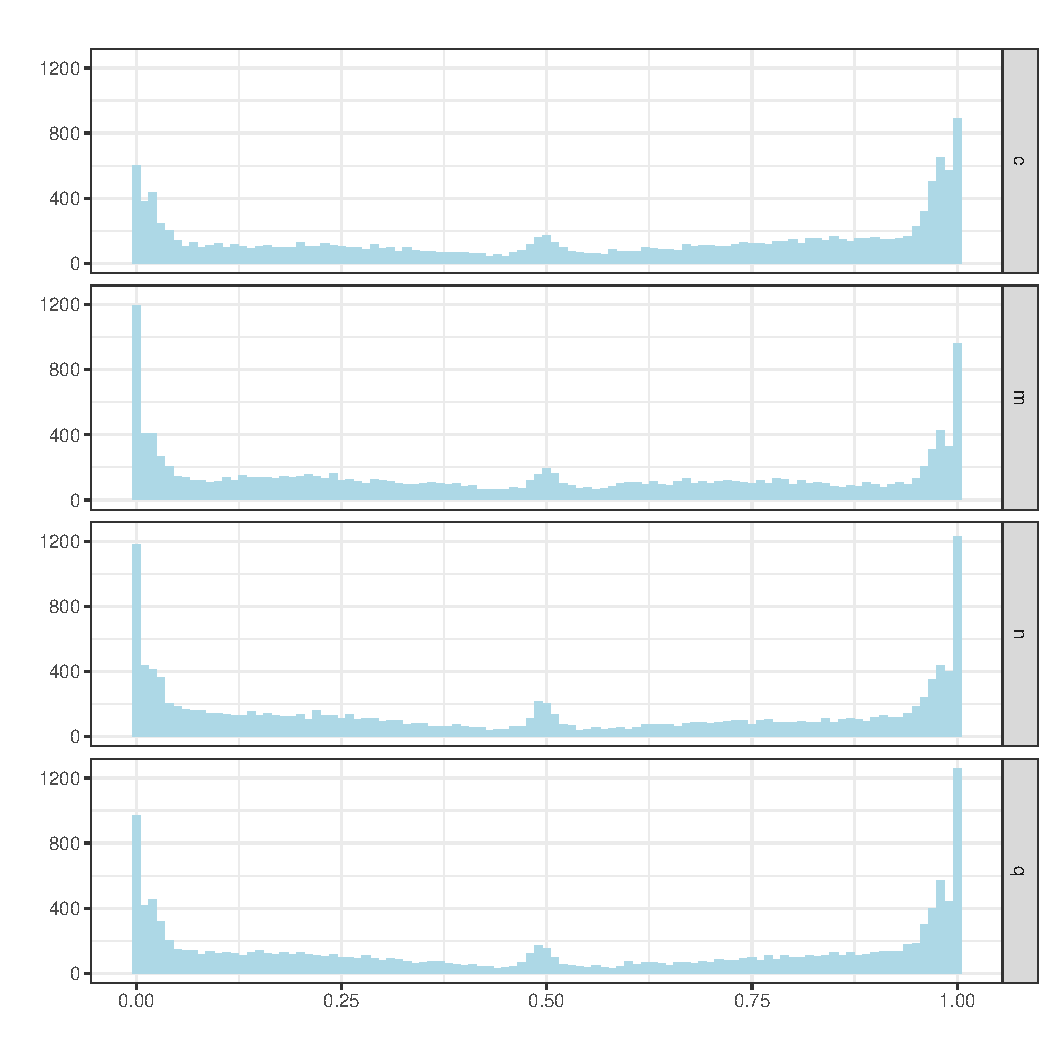
\includegraphics[width=\linewidth]{figures/figuresproject-by-op-distr-1} 

}


\end{knitrout}

\begin{itemize}
  \item These definitely do not look normal
  \item Maybe a beta-regression would be useful?
  \item But even that would be relying on some simplifying assumptions, since we might be ignoring the little bump in the middle 
\end{itemize}

\newpage
\subsection{Distribution of projectivity ratings by verb:}
\begin{knitrout}
\definecolor{shadecolor}{rgb}{0.969, 0.969, 0.969}\color{fgcolor}

{\centering 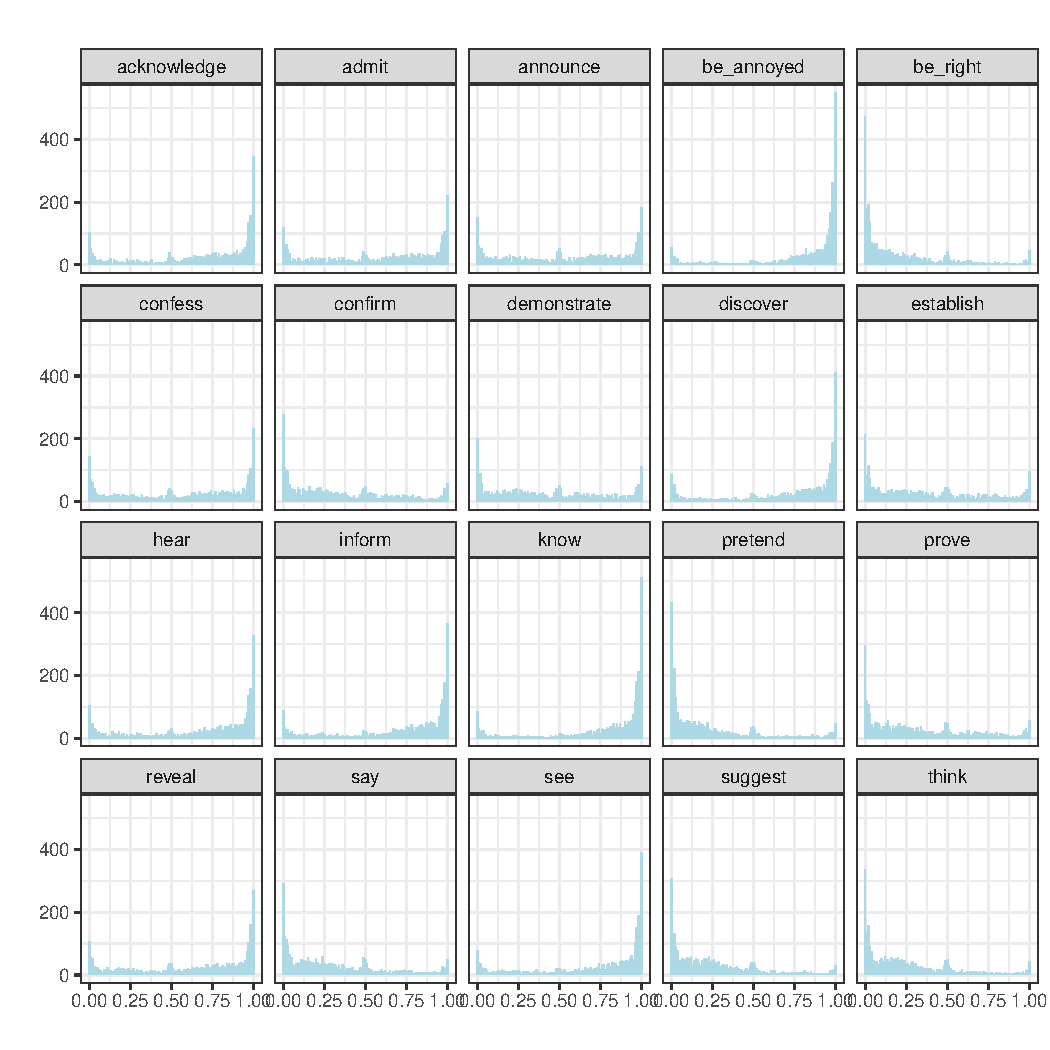
\includegraphics[width=\linewidth]{figures/figuresproject-by-v-distr-1} 

}


\end{knitrout}

\begin{itemize}
  \item Some of these also show a higher mass around the middle of the scale
  \item but it looks the beta-distribution could be useful
\end{itemize}


\newpage
\subsection{Means and confidence intervals for projectivity rating by operator}
\begin{knitrout}
\definecolor{shadecolor}{rgb}{0.969, 0.969, 0.969}\color{fgcolor}

{\centering 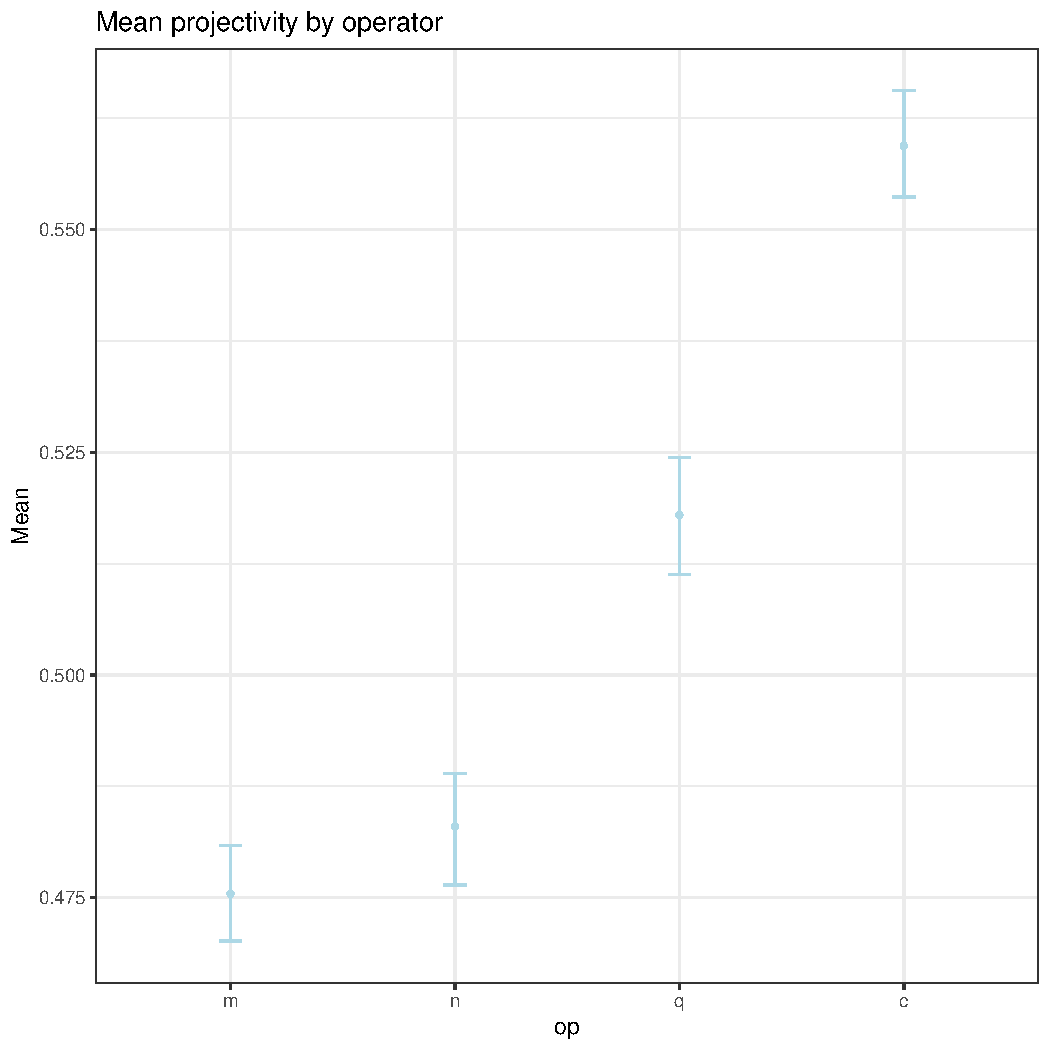
\includegraphics[width=.6\textwidth]{figures/figuressummary-op-1} 

}


\end{knitrout}

\noindent The following generalizations emerge:
\begin{itemize}
  \item Conditionals have the highest projectivity ratings
  \item Projectivity ratings for questions are higher than those for modals and negation, but lower than those for conditionals
  \item Modals and negation have the lowest projectivity ratings
  \item The ratings for negation look a little higher than for modals, but error bars overlap
\end{itemize}

\noindent Although these differences appear to be significant, they are quite small.\\

\newpage
\subsection{Means and confidence intervals for projectivity rating by verb:}
This will be replaced by violin-plot.
% <<summary-v, echo = FALSE, message=FALSE, cache=TRUE, fig.width=14, fig.height=7>>=
% 
% proj_means_v = data %>% group_by(verb) %>%
%   summarize(Mean = mean(projective), CILow = ci.low(projective),
%             CIHigh = ci.high(projective)) %>%
%   mutate(YMin = Mean - CILow, YMax = Mean + CIHigh,
%          verb = fct_reorder(as.factor(verb),Mean)) %>% ungroup()
% 
% proj_means_v %>% mutate(verb = fct_reorder(verb, Mean,
%                                          .fun = mean)) %>%
%   ggplot(aes(x=verb, y=Mean)) +
%   coord_cartesian(ylim=c(0,1)) +
%   geom_point(color = "lightblue") +
%   geom_errorbar(aes(ymin=YMin,ymax=YMax), width=0.1, color = "lightblue") +
%   labs(title = "Mean projectivity by predicate")+
%   theme_bw()
% @
\begin{itemize}
  \item We see gradual differences in projectivity between verbs
\end{itemize}

\subsection{Means and confidence intervals for projectivity rating by verb and operator:}
\begin{knitrout}
\definecolor{shadecolor}{rgb}{0.969, 0.969, 0.969}\color{fgcolor}

{\centering 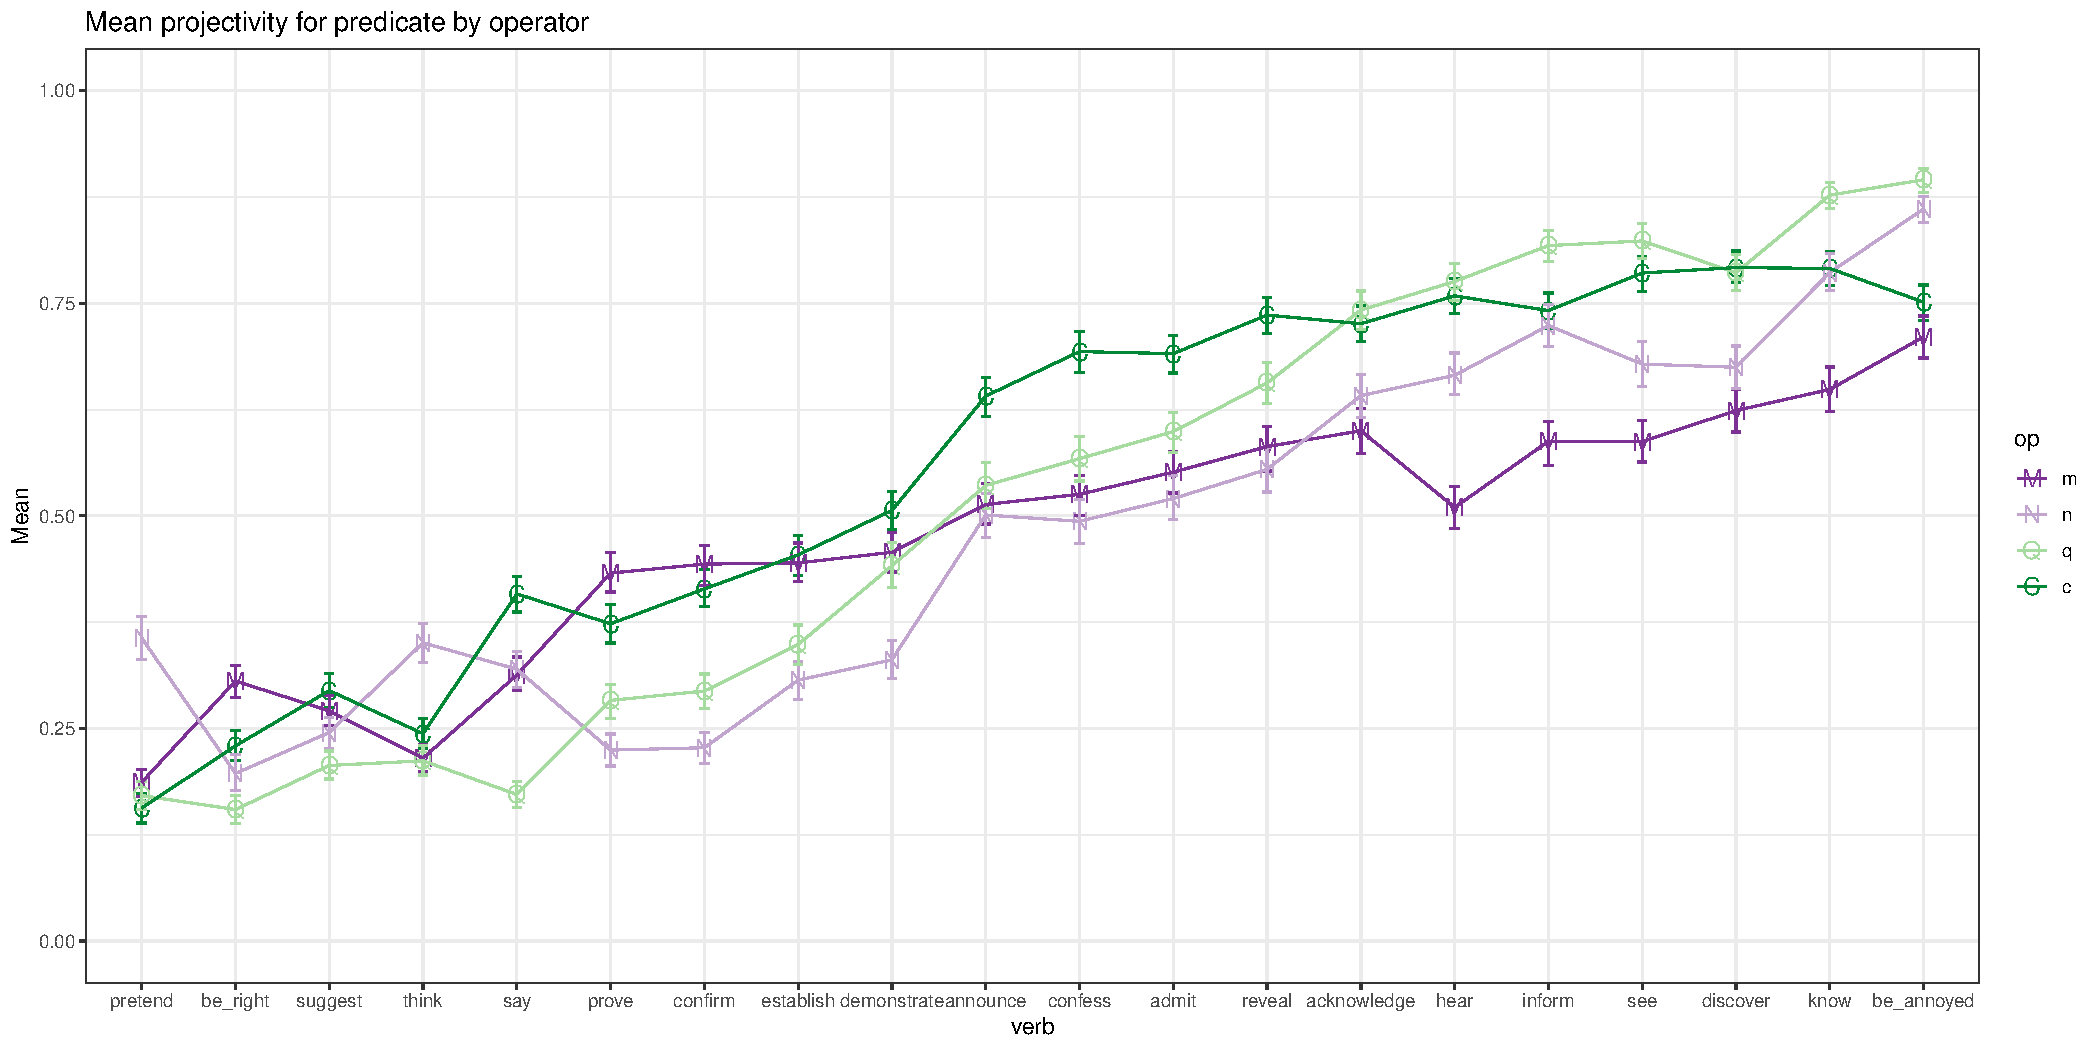
\includegraphics[width=\linewidth]{figures/figuressummary-combined-1} 

}


\end{knitrout}

\begin{itemize}
  \item We see interactions between verb and operator

  \item Two verbs show highest projectivity under negation: the anti-veridical \emph{pretend}, and the non-veridical \emph{think}. These are verb with relatively low overall projectivity.

  \item More projective verbs (\emph{\lq announce\rq} and above) have $\texttt{C} > \texttt{M}$

  \item Highly projective verbs (\emph{\lq hear \rq} and above) have  $\texttt{N} > \texttt{M}$

  \item We do not see any group of verbs that could be characterized as \lq semi-factive\rq\ in the sense of Karttunen.
  \begin{itemize}
    \item Specifically, \emph{discover} does not follow the predicted pattern: It is not more projective under negation, but most projective in conditionals and questions.
    \item For Karttunnen's \lq factives\rq, no difference between operators is expected.
    \item Kajsa Djärv about this distinction: cognitive predicates are semi-factive, and emotives are factive. The pattern suggested by karrtunen is also not found here
  \end{itemize}

  \item For more generalizations, let's look at the same information plotted differently: By-operator projectivity for each verb
\end{itemize}


\begin{knitrout}
\definecolor{shadecolor}{rgb}{0.969, 0.969, 0.969}\color{fgcolor}

{\centering 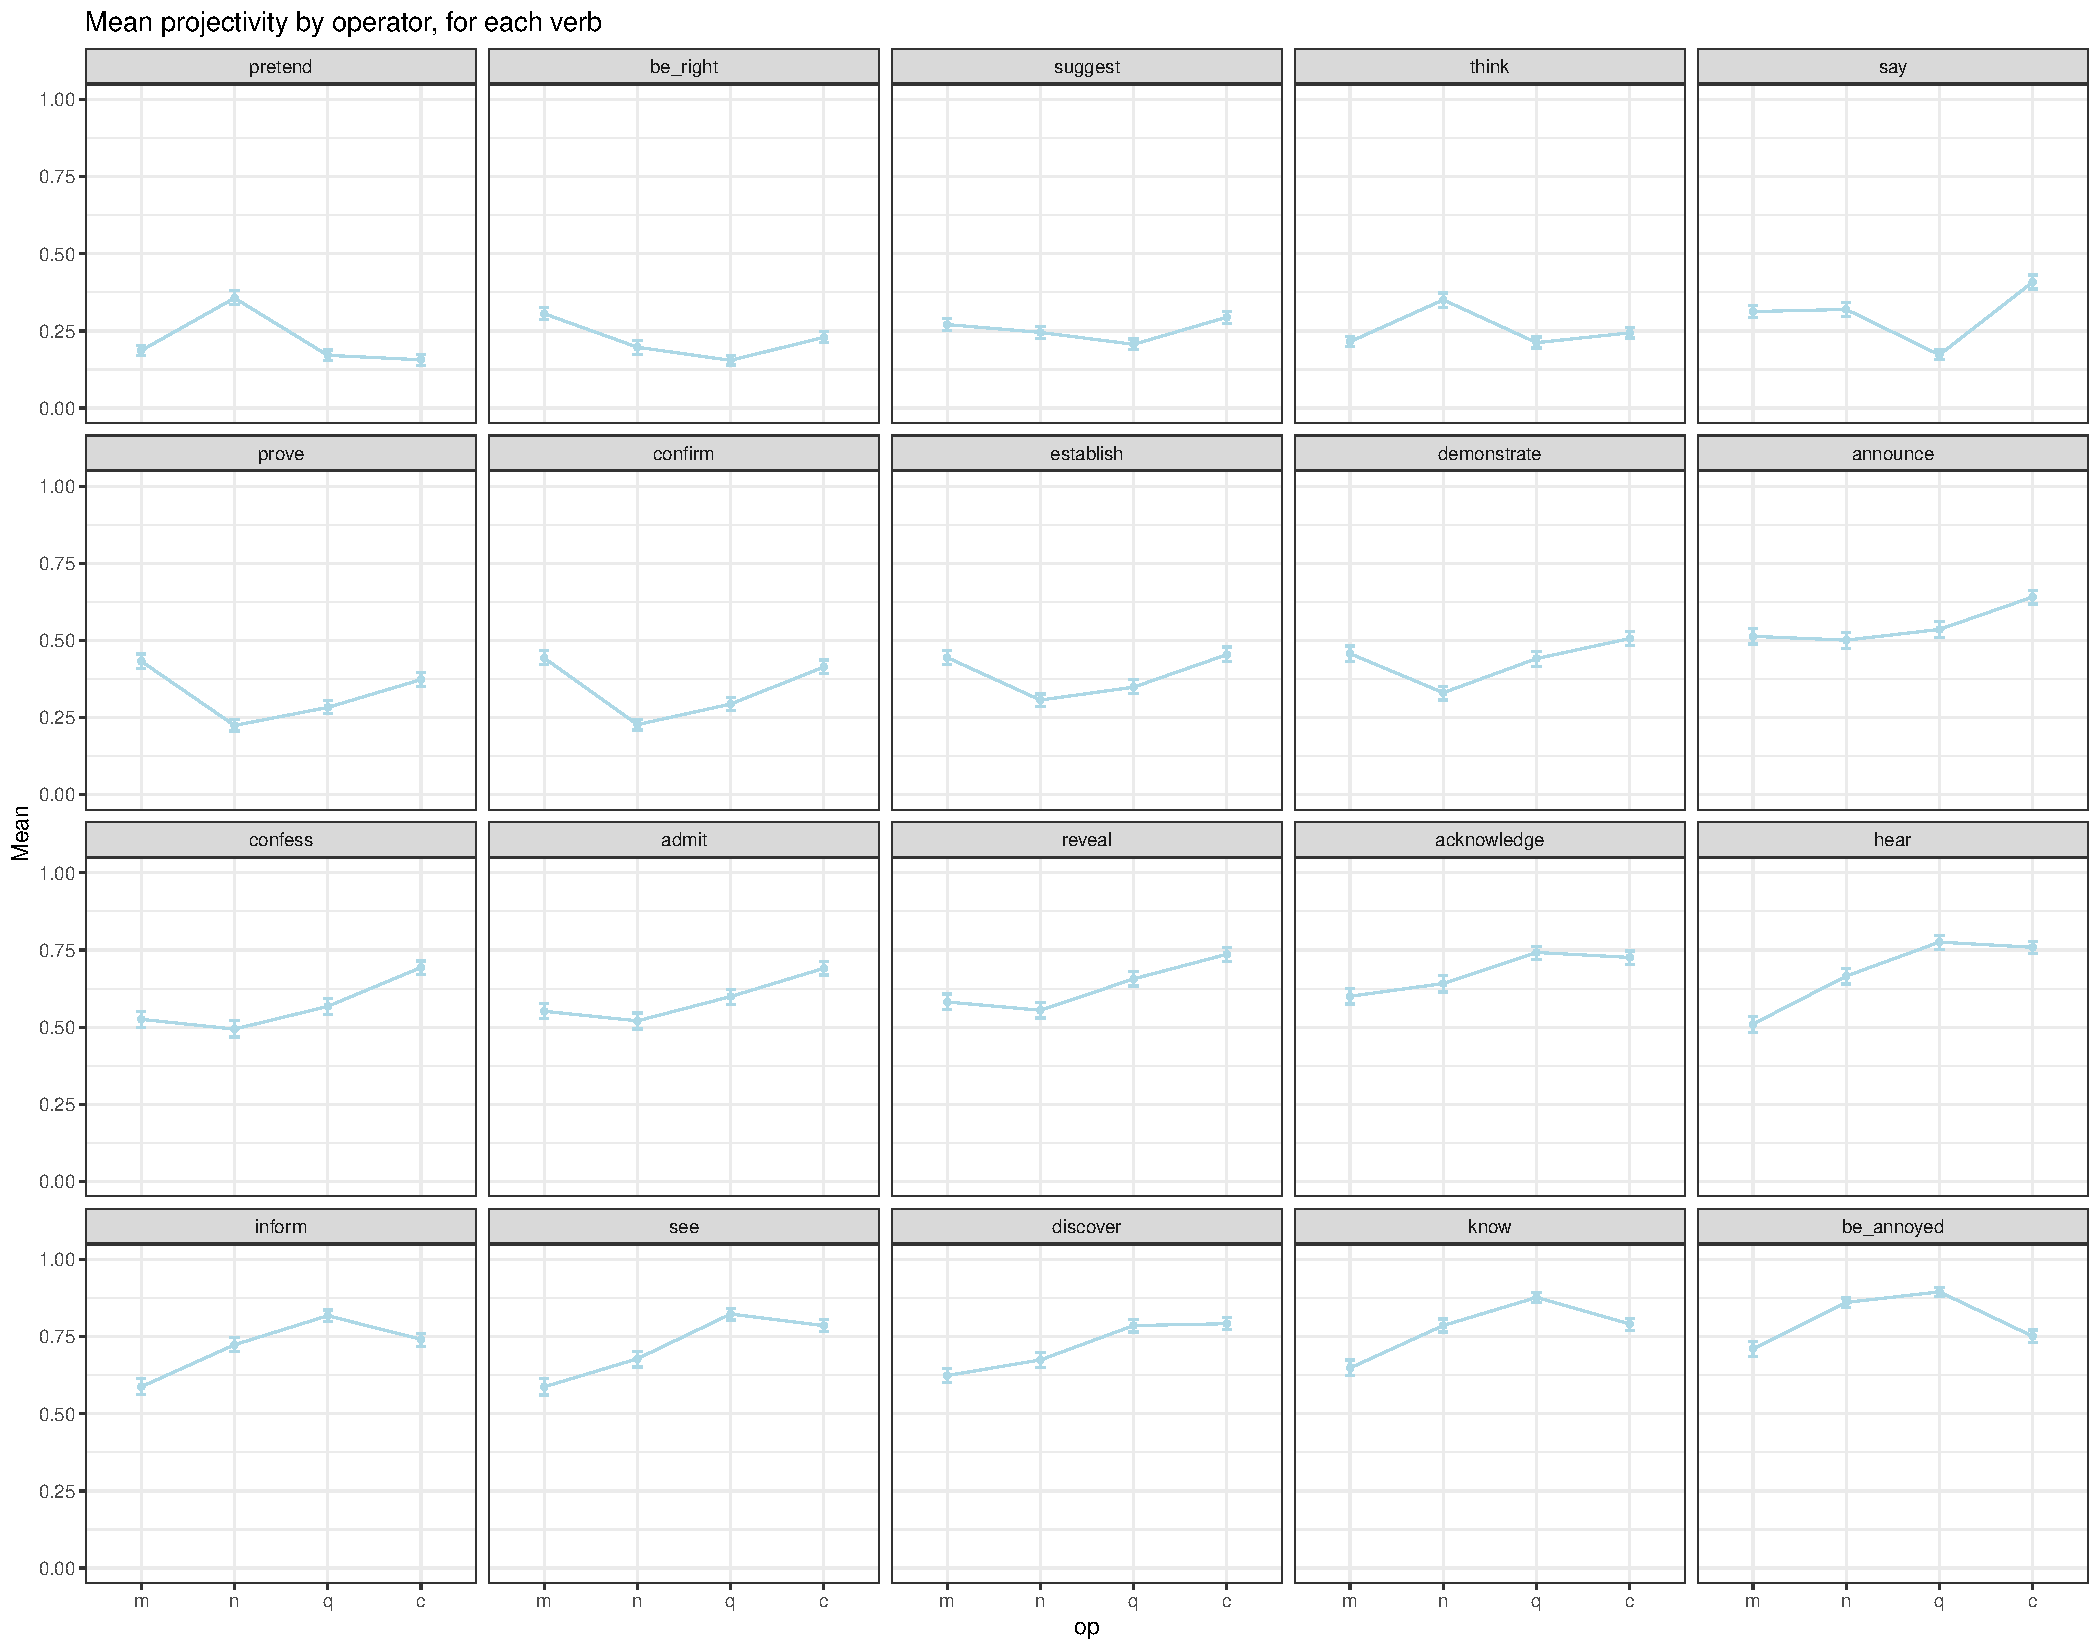
\includegraphics[width=\linewidth]{figures/figuresverb-profiles-1} 

}


\end{knitrout}
Some more generalizations: We find different \lq profiles\rq for different verbs, of how embedding operators affect projectivity based on the verb. Groups of verbs show similar profiles:

\begin{itemize}
  \item \emph{pretend, think}: \textbf{anti-veridical profile}\\
    \texttt{N} $>$ \texttt{M, Q, C}, overall low projectivity

  \item \emph{acknowledge, hear, inform, see, discover, know, be annoyed}: \textbf{\lq factive\rq profile}\\
    \texttt{Q} $>$ \texttt{N, C} \textcolor{gray}{$>_?$} \texttt{M}, overall high projectivity (it may be possible to find further subgroups here)

  \item \emph{prove, confirm, establish, demonstrate, (announce), confess, admit, reveal}: \textbf{veridical profile}\\
    \texttt{M, C} $>$ \texttt{Q} $>$ \texttt{N}, overall med-lo to med-hi projectivity
  
  \item \emph{be right, suggest}: \textbf{reportative profile}\\
    \texttt{M, N, C} $>$ \texttt{Q}

\end{itemize}

Maybe these can have better names, not trying to suggest that verbs can neatly divided in factive v non-factive, but potentially this class / profile is what prompted intuitions in previous literature, and naming in this tradition could make sense, but can be changed depending on our rhetoric, of course.

% \section{Analysis}
% 
% We are interested in how the response (projectivity ratings) depends on the verb and embedding operator, and whether the above generalizations can be supported statistically.
% 
% 
% 
% <<>>=
% formula <- response ~ op * verb
% # formula <- response ~ op * verb + (1 | workerid) + (1 | item)
% # formula <- response ~ op * verb + (1 + op + verb | workerid) + (1 + op + verb | item)
% @
% 
% Trying a beta-regression. Our response variable has observations from a sliding scale between $(0,1)$. For beta regression, we rescale it to $[0,1]$, using method used in Degen \& Tonhauser (2022), from Smithson \& Verkuilen (2006).
% 
% <<>>=
% data$response = (data$projective*(nrow(data)-1) + .5)/nrow(data)
% @
% 
% 
% <<>>=
% # library(rstan)
% # options(mc.cores=parallel::detectCores())
% # rstan_options(auto_write=TRUE)
% # library(brms)
% # 
% # model1 <- brm(formula = bf(response ~ op * verb ,
% #                            phi ~ op * verb,
% #                            family = Beta()),
% #               family = Beta(),
% #               data = data,
% #               iter=10000, warmup=2000,chains=6)
% 
% 
% @
% 
% 


\end{document}


